Date : 1 december 2023

\subsubsection{Overdracht}

Een elektromagnetische golf plant zich voor in vacuüm(ether) met de
lichtsnelheid.
In een kabel (koper/optisch) plant de golf zich met een lagere snelheid voort
dan de lichtsnelheid.
\begin{itemize}[label=$\bullet$]
    \item Een EM golf bestaat uit een elektrisch en magnetisch veld.
    \item Het elektrische en magnetische veld staan loodrecht ten opzichte van elkaar.
    \item De richting van het elektrische veld wordt    de polarisatierichting genoemd.
    \item labda = c/f
  \end{itemize}

\begin{figure}[H]
\centering
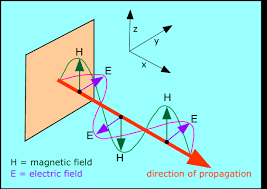
\includegraphics[scale=0.8]{EM signaal.png}
\caption{EM Signaal.}
\end{figure}

\begin{figure}[H]
\centering
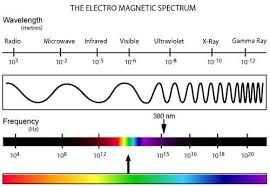
\includegraphics[scale=0.8]{elektromagnetisch spectrum.jpeg}
\caption{Elektromagnetisch spectrum}
\end{figure}


\subsubsection{Golflengte}

Voortplantingssnelheid in de vrije ruimte, wordt lichtsnelheid ‘c’
genoemd en is 3.108 m/s. 
Het verband tussen de golflengte en de frequentie: labda = c/f

\begin{figure}[H]
\centering
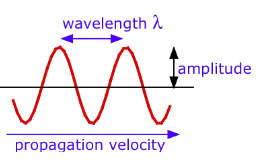
\includegraphics[scale=0.8]{Golflengte.png}
\caption{Golflengte}
\end{figure}

\subsubsection{Verkortingsfactor}

De voorplantingssnelheid in een medium. Dus bijvoorbeeld een kabel
of fiber is lager.\\
in vacuum geldt \(c = \sqrt{\frac{1}{\varepsilon_0 \mu_0}}\)\\
waarin \(\varepsilon_0\) de elektische veldconstante is\\
waarin \(\mu_0\) de magnetische veldconstante is\\

In een kabel zijn deze constanten hoger waardoor de snelheid lager wordt. Deze verlaging wordt de Verkortingsfactor genoemd. De Verkortingsfactor van bijvoorbeeld een coaxkabel is 2/3.\\

Een Verkortingsfactor heeft  gevolgen voor de golflengte in de kabel! Je moet hier bij de volgende zaken rekening mee houden:
\begin{itemize}[label=$\bullet$]
    \item Board design, lengte van printsporen
    \item Antenne-afmetingen
    \item Lichtbreking (fiber communication)
\end{itemize}

\subsubsection{Impedantie}

De impedantie (\(Z\)) wordt gegeven door de som van de reële component (\(R\)), ook wel de weerstand genoemd, en de imaginaire component (\(jX\)), ook wel reactantie genoemd. Deze reactantie kan inductief of capacitief zijn.

\[
Z = R + jX
\]

Waarbij:
\begin{align*}
R & : \text{Reële component (weerstand)} \\
jX & : \text{Imaginaire component (reactantie)}
\end{align*}

De karakteristieke impedantie (\(Z_0\)) van een kabel of vierpool is de impedantie die aan de ingang gelijk wordt aan de impedantie waarmee je de uitgang afsluit. Wanneer je hieraan voldoet, heb je op alle punten de juiste aanpassing en dus optimale vermogensoverdracht!

\[
Z_0
\]

Zkar van een kabel: \\
Een klein stukje kabel is voor te stellen als een vierpool:
\begin{figure}[H]
\centering
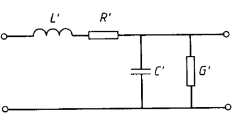
\includegraphics[scale=0.8]{vierpool.png}
\caption{Vierpool}
\end{figure}
Voor een verliesvrije kabel geldt R=0 en G=oneindig
\[
Zkar = \sqrt{L / C}
\]

\subsubsection{Afsluiten van transmissielijnen}

We willen een maximale vermogensoverdracht van een bron naar een belasting bereiken wanneer de impedantie van de bron (\(Z_i\)) gelijk is aan de impedantie van de belasting (\(Z_l\)). Wanneer dit niet het geval is, treedt bij hoogfrequente signalen reflectie op.

Deze situatie heeft twee ongewenste gevolgen:
\begin{enumerate}
  \item Vermogensverlies
  \item Mogelijke beschadiging van de zender (eindtrap) door extra dissipatie van gereflecteerd vermogen. Dit kan leiden tot oververhitting. Meer geavanceerde systemen zijn vaak beschermd tegen dergelijke situaties.
\end{enumerate}

karakteristiek korgesloten = Alle energie komt terug. De spanning wordt gereflecteerd in tegenfase.
\begin{figure}[H]
\centering
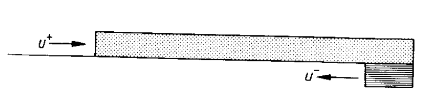
\includegraphics[scale=0.8]{karakteristiek kortgesloten.png}
\caption{karakteristiek kortgesloten}
\end{figure}

karakteristiek open = Alle energie komt terug. De spanning wordt gereflecteerd in fase.
\begin{figure}[H]
\centering
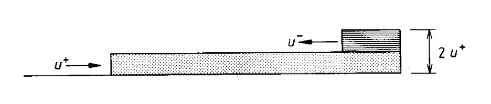
\includegraphics[scale=0.8]{karakteristiek open.png}
\caption{karakteristiek open}
\end{figure}

\subsubsection{Pulsechometing}

Pulseecho-metingen of een Optical Time Domain Reflectometer (OTDR) worden gebruikt bij glasvezelkabels. Op de positie van de breuk bevindt zich in feite een open uiteinde (de energie komt terug!). Door de tijd te meten tussen de verstuurde en gereflecteerde puls is de positie van de breuk vast te stellen! De essentiële parameter van een kabel die hiervoor nodig is, is de verkortingsfactor; deze bepaalt de snelheid van de elektromagnetische golf in de kabel (\(c\)).

\subsubsection{decibel}
\begin{figure}[H]
\centering
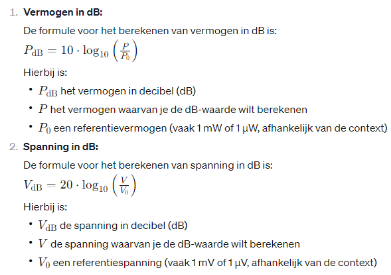
\includegraphics[scale=1.1]{vermogen.png}
\end{figure}

\begin{itemize}
    \item Wat is dBm? 
    \[ \text{dBm} = 10 \cdot \log_{10}\left(\frac{P}{1 \, \text{mW}}\right) \]
  
    \item Wat is dBi? 
    \begin{itemize}
      \item Decibels ten opzichte van een isotrope straler.
      \item Isotrope straler? (Komen we nog op terug)
    \end{itemize}
  
    \item En dBd? 
    \begin{itemize}
      \item Decibels ten opzichte van een dipool. (Komen we ook nog op terug)
    \end{itemize}
  \end{itemize}
